\begin{table}[H]
	\captionsetup{labelformat=empty}
	\centering
	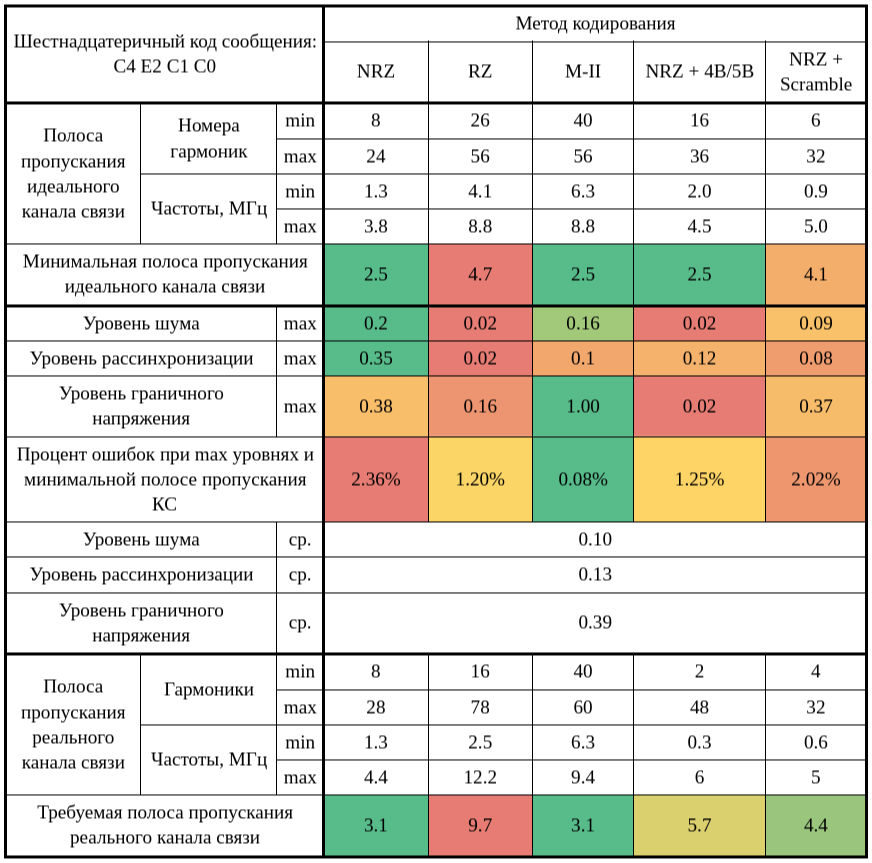
\includegraphics[width=1\textwidth]{./data/comp_table.png}
	\caption{Таблица 2.1}
\end{table}

Хуже всего себя показал RZ. Он обладает худшей устойчивостью к помехам, хотя и дает средний результат по количеству ошибок при максимальных уровнях помех. Также он имеют наибольшую ширину требуемой полосы пропускания реального канала связи, и, в отличие от остальных методов, имеет три уровня потенциала, что увеличивает стоимость его реализации.

Наименьшую ширину полосы пропускания реального канала связи имеет NRZ (3.1 МГц). Однако, он обладает недостатками потенциального метода кодирования: у NRZ отсутствует самосинхронизация, что может привести к рассинхронизации и некорректной интерпретации данных на приемнике; а также при передаче последовательностей нулей или единиц его невозможно использовать в электрических каналах связи при наличии гальванических развязок. К тому же, NRZ показал наибольший процент ошибок при помехах (2.16\%).

Проблемы NRZ решает логическое кодирование – NRZ+4B/5B и NRZ+Scramble. Эти методы улучшают свойства самосинхронизации, позволяют выявлять ошибки и избавляют NRZ от постоянной составляющей. Но их недостатком является увеличенная полоса пропускания реального канала связи (5.7 и 4.4 МГц соответственно), а также они имеют средний результаты по допустимым уровням помех и проценту ошибок.

\underline{Лучше всех оказался \textbf{M2}}. При одинаковой с NRZ полосой пропускания реального канала связи (3.1 МГц), он показал один из лучшие результатов среди всех методов по допустимым уровням помех, он абсолютно устойчив к уровню граничного напряжения, а также Манчестер имел наименьший процент ошибок при совмещении различного рода помех (0.08\%).

Также, по сравнению с NRZ, он:
\begin{enumerate}
	\item Не имеет постоянной составляющей, что необходимо для поддержки синхронизации, а также для корректной работы трансформаторных схем гальванической развязки;
	\item Обладает свойством самосинхронизацией, что решает проблемы синхронизации, и исключает пропуск или повторное считывание бита.
\end{enumerate}
